\chapter{Východiská práce}
\label{kap:vychodiska} % id kapitoly pre prikaz ref

V tejto kapitole sa čitateľ oboznámi zo základnými princípami logiky prvého rádu ktoré sú nevyhnutné na pochopenie práce. Zistí, aké prostriedky a technológie boli použité na vývoj aplikácie. Na záver je krátka analýza existujúcich prác a aplikácií, ktoré ma určitým spôsobom inšpirovali pri tvorbe.

\section{Logika prvého rádu}
Logika prvého rádu je formálny systém používaný v matematike a informatike. Od jednoduchej výrokovej logiky sa odlišuje tým, že pridáva predikáty a kvantifikátory. Nasledujúce definície v tejto kapitole vychádzajú z prednášok \cite{prednasky} a Švejdarovej učebnice \cite{svejdar}.


\subsection{Jazyk}
Jazyk $\mathcal{L}$ v prvorádovej logike je formálny jazyk ktorý definuje množinu konkrétnych symbolov, ktoré definujú syntax a sémantiku logiky. Jazyk obsahuje logické symboly, symboly indivíduových premenných, mimologické symboly a pomocné symboly.

\paragraph{}
Medzi \emph{logické symboly} patria logické spojky ($\vee, \wedge, \to, \neg$), symbol rovnosti ($\doteq$) a kvantifikátory ($\forall, \exists$).

\paragraph{}
\emph{Symboly indivíduových premenných} sú symboly z nejakej nekonečnej spočítateľnej množiny $\mathcal{V}_\mathcal{L}$ a predstavujú niečo nekonkrétne. Príklad definovania množiny symbolov premenných v jazyku je v \ref{eq:definovanie_vl}.
\begin{equation} \label{eq:definovanie_vl}
\mathcal{V}_\mathcal{L} = \{x, y, z, ...\}
\end{equation}

\paragraph{}
Medzi \emph{mimologické symboly} patria \emph{symboly konštánt} $\mathcal{C}_\mathcal{L}$, \emph{funkčné symboly} $\mathcal{F}_\mathcal{L}$ a \emph{predikátové symboly} $\mathcal{P}_\mathcal{L}$. Všetkým predikátovým a funkčným symbolom je priradená \emph{arita}. Arita je kladné prirodzené číslo a predstavuje počet argumentov symbolu. Arita sa zapisuje ako horný pravý index pri názve symbolu. Napríklad \texttt{nenávidí}$^2$ je predikátový symbol s aritou 2.

\paragraph{}
Symbol konštanty z množiny $\mathcal{C}_\mathcal{L}$ jazyka $\mathcal{L}$ predstavuje konkrétny objekt ktorý sa nedá zameniť alebo konkrétnu hodnotu. Dá sa povedať, že sú podobné ako vlastné mená v prirodzenom jazyku alebo konštanty v programovacom jazyku. Napríklad symbol konštanty \texttt{Dom123} predstavuje konkrétny dom s číslom 123 v nejakej obci a nedá sa zameniť zo žiadnym iným. Príklad definovania množiny konštánt v jazyku je v \ref{eq:definovanie_cl}.
\begin{equation} \label{eq:definovanie_cl}
\mathcal{C}_\mathcal{L} = \{\texttt{Dom123}, \texttt{Frantisek}, \texttt{Velkost}\}
\end{equation}

\paragraph{}
Funkčný symbol z množiny $\mathcal{F}_\mathcal{L}$ jazyka $\mathcal{L}$ predstavuje jednoznačne určený vzťah.Napríklad funkčný symbol \texttt{cena(Produkt123)} predstavuje cenu produktu 123 v nejakom obchode. Produkt bežne máva iba jednu cenu, takže \texttt{Produkt123} má nejakú \emph{jednoznačne} určenú cenu. Príklad definovania množiny funkčných symbolov v jazyku je v \ref{eq:definovanie_fl}.
\begin{equation} \label{eq:definovanie_fl}
\mathcal{F}_\mathcal{L} = \{\texttt{cena}^1, \texttt{-}^2\}
\end{equation}

\paragraph{}
Predikátový symbol z množiny $\mathcal{P}_\mathcal{L}$ jazyka $\mathcal{L}$ predstavuje určitú vlastnosť alebo vzťahy. Príklad definovania množiny predikátových symbolov v jazyku je v \ref{eq:definovanie_pl}.
\begin{equation} \label{eq:definovanie_pl}
\mathcal{P}_\mathcal{L} = \{\texttt{nenávidí}^2, \texttt{chlapec}^1\}
\end{equation}

\paragraph{}
Množiny $\mathcal{V}_\mathcal{L}, \mathcal{P}_\mathcal{L}, \mathcal{F}_\mathcal{L}, \mathcal{C}_\mathcal{L}$ sú navzájom disjunktné. Medzi \emph{pomocné symboly} patria \texttt{'(', ')' a ','}



\subsection{Syntax}

\paragraph{}
\emph{Termy} jazyka $\mathcal{L}$ predstavujú konkrétne (pomenované symbolmi konštánt) alebo nekonkrétne (pomenované symbolmi premenných) objekty. Ak $t_1$ až $t_n$ sú termy, a $f$ je funkčný symbol s aritou $n$, tak aj $f(t_1, .., t_n)$ je term. Pre jazyk $\mathcal{L}$ sú preto tieto termy:
\begin{itemize}
	\item nekonkrétne - $\texttt{x}, \texttt{y}, \texttt{z}$
	\item konkrétne - $\texttt{Frantisek}, \texttt{Dom123}, \texttt{Velkost}$
	\item vzťahy - $\texttt{cena(x)}, \texttt{cena(Dom123)}, \texttt{-(x,y)}, ...$
\end{itemize}

\paragraph{}
\emph{Atomické formuly} jazyka $\mathcal{L}$ je množina $\mathcal{A}_\mathcal{L}$. Medzi atomické formuly patrí \emph{rovnostný atóm} a \emph{predikátový atóm}. Ak $t_1$ až $t_n$ sú termy, tak postupnosť symbolov $t_1 \doteq t_2$ sa nazýva rovnostný atóm jazyka $\mathcal{L}$. Rovnostné atómy vyjadrujú, že dva termy ukazujú na ten istý objekt. Ak $t_1$ až $t_n$ sú termy a $P$ je predikátový symbol s aritou $n$, tak postupnosť symbolov $P(t_1, ..,  t_n)$ sa nazýva predikátový atóm jazyka $\mathcal{L}$. 

\paragraph{}
Množina \emph{formúl} jazyka $\mathcal{L}$ je induktívne definovaná nasledovne:
\begin{itemize}
    \item všetky atomické formuly sú formulami
    \item ak sú $\alpha$ a $\beta$ formuly, tak aj $(\alpha \wedge \beta)$, $(\alpha \vee \beta)$, $(\alpha \to \beta)$, $\neg \alpha$ sú formulami
    \item ak $x$ je indivíduová premenná a $\alpha$ je formula, tak aj $\forall x \alpha$ a $\exists x \alpha$ sú formulami
\end{itemize}


\subsection{Sémantika}
\paragraph{}
Hodnota formuly alebo termu jazyka $\mathcal{L}$ určuje \emph{štruktúra}. Štruktúrou pre jazyk $\mathcal{L}$ je dvojica $\mathcal{M} = (M, i)$, kde $M$ je doména štruktúry a $i$ je interpretačná funkcia štruktúry.

\paragraph{}
\emph{Doména} štruktúry je množina symbolov objektov na ktoré ukazujú termy.

\paragraph{}
\emph{Interpretačná funkcia} je zobrazenie, ktoré každému symbolu konštanty $c$ jazyka $\mathcal{L}$ priraďuje prvok $i(c) \in M$, každému funkčnému symbolu $f$ jazyka $\mathcal{L}$ s aritou $n$ priraďuje funkciu $i(f): M^n \to M$ a každému predikátovému symbolu $P$ jazyka $\mathcal{L}$ s aritou $n$ priraďuje množinu $i(P) \subseteq M^n$.

\paragraph{}
\emph{Ohodnotenie (indivíduových) premenných} jazyka $\mathcal{L}$ je ľubovoľná funkcia $e: \mathcal{V}_\mathcal{L} \to M$ ktorá každej premennej priraďuje prvok z domény.

\paragraph{}
\emph{Hodnotou termu t} v štruktúre $\mathcal{M}$ pri ohodnotení premenných \emph{e} je prvok $t^\mathcal{M}[e]$ z \emph{M} určený nasledovne:
\begin{itemize}
	\item $x^\mathcal{M}[e] = e(x)$, ak $x$ je premenná,
	\item $a^\mathcal{M}[e] = i(a)$, ak $a$ je konštanta,
	\item $(f(t_1, .., t_n))^\mathcal{M}[e] = i(f)(t_1^\mathcal{M}[e], .., t_n^\mathcal{M}[e])$, ak $t_1, .., t_n$ sú termy.
\end{itemize}

\paragraph{}
Relácia \emph{štruktúra $\mathcal{M}$ spĺňa formulu A pri ohodnotení e} (skrátene $\mathcal{M} \models A[e]$) má nasledovnú induktívnu definúciu:
\begin{itemize}
	\item $\mathcal{M} \models t_1 \doteq t_2[e]$ vtt $t_1^\mathcal{M}[e] = t_2^\mathcal{M}[e]$,
	\item $\mathcal{M} \models P(t_1, .., t_n)[e]$ vtt $(t_1^\mathcal{M}[e], .., t_n^\mathcal{M}[e]) \in i(P)$,
	\item $\mathcal{M} \models \neg A[e]$ vtt $\mathcal{M} \not\models A[e]$,
	\item $\mathcal{M} \models (A \wedge B)[e]$ vtt $\mathcal{M} \models A[e]$ a zároveň $\mathcal{M} \models B[e]$,
	\item $\mathcal{M} \models (A \vee B)[e]$ vtt $\mathcal{M} \models A[e]$ alebo $\mathcal{M} \models B[e]$,
	\item $\mathcal{M} \models (A \to B)[e]$ vtt $\mathcal{M} \not\models A[e]$ alebo $\mathcal{M} \models B[e]$,
	\item $\mathcal{M} \models \exists xA[e]$ vtt pre \emph{nejaký} prvok $m \in M$ máme $\mathcal{M} \models A[e(x/m)]$,
	\item $\mathcal{M} \models \forall xA[e]$ vtt pre \emph{každý} prvok $m \in M$ máme $\mathcal{M} \models A[e(x/m)]$,
\end{itemize}
pre všetky arity $n > 0$, všetky predikátové symboly $P$ s aritou $n$, všetky termy $t_1, t_2, .., t_n$, všeky premenné $x$ a všetky formuly $A, B$.

\paragraph{}
Formula \emph{A} je \emph{splniteľná} vtt aspoň jedna štruktúra $\mathcal{M}$ pre jazyk $\mathcal{L}$ spĺňa \emph{A} pri aspoň jednom ohodnotení \emph{e}.





\section{Analýza použitých technológií}
\paragraph{}
V tejto sekcii sa čitateľ oboznámi s technológiami ktoré budú použité pri tvorbe aplikácie. 


\subsection{Javascript, HTML, CSS, Bootstrap}
\paragraph{}
\emph{Javascript} je objektovo orientovaný, interpretovaný programovací jazyk využívaný hlavne vo webových aplikáciách. Väčšinou sa vykonáva na strane klienta (webový prehliadač) a reaguje na rôzne udalosti od užívateľa (napr. kliknutie myšou na nejaký element, zmenšenie okna a podobne). Vďaka tomuto je možné vytvárať dynamické a interaktívne webové aplikácie.

\paragraph{}
\emph{HTML} je značkovací jazyk využívaný na tvorbu webových stránok a webových aplikácií. Definuje tagy, pomocou ktorých sa formátuje text, pridávajú obrázky alebo vytvárajú hypertextové linky na iné stránky. Webový server posiela HTML súbory ako odpoveď na požiadavku do webového prehliadača, ktorý dokáže tieto značky správne vyrenderovať. V čase vývoja tejto aplikácie bol štandard HTML5.2 a všetky definície vychádzajú z \cite{html}

\paragraph{}
\emph{CSS} je štýlovací jazyk na štýlovanie HTML elementov. Tento jazyk využijem na vizuálne rozloženie a štýlovanie elementov v aplikácii (tlačidlá, text, ...).

\paragraph{}
\emph{Bootstrap} je moderný, veľmi využívaný CSS a Javascript framework na štýlovanie webovej stránky. Má (okrem iného) predvytvorené mechanizmy ako rozložiť elementy na stránke pre rôzne rozlíšenia prehliadača - tzv. grid. Tento framework využijem na rozloženie stránky. 



\subsection{React}
React je Javascript knižnica vytvorená spoločnosťou Facebook, Instagram a komunitou vývojárov. Originálnym autorom je vývojár v spoločnosti Facebook, Jordan Walke. Prvá verzia React-u vyšla v marci v roku 2013 \cite{wiki:react}. 
\paragraph{}
Hlavným cieľom tejto knižnice je efektívna tvorba používateľských rozhraní. V tejto kapitole sa budem snažiť v krátkosti opísať architektúru React-u na príklade, kde budem vytvárať rozhranie na pridávanie textových reťazcov do zoznamu. Nechcem zachádzať do detailov, budem v krátkosti opisovať iba tie veci, ktoré využijem pri tvorbe aplikácie. Ukážky kódov sú zjednodušené, aby boli ľahšie čitateľné. Zdrojom k tejto sekcii je hlavná, online dokumentácia React-u \cite{man:react}.

\subsubsection{Elementy a komponenty}
React je vo všetkých smeroch Javascriptová knižnica. Nekombinujú sa v nej HTML a Javascript súbory ako je to pri klasických MVC frameworkoch. V aplikáciách tvorené cez React sa stránky nevytvárajú pomocou klasických HTML súborov kde sa píšu HTML elementy, ale namiesto toho sa vytvárajú Javascript \emph{objekty} HTML elementov. Objekt elementu obsahuje typ, atribúty a potomkov, ktoré by mal štandardný HTML element. Napríklad element \texttt{<button>} môže obsahovať atribúty \texttt{id}, \texttt{class}, \texttt{style} a iné. Elementy môžu mať tiež ľubovoľný počet potomkov.
\paragraph{}
\emph{Element} v React-e je objektová reprezentácia HTML elementu. Každý element má definovaný typ, atribúty a zoznam potomkov, ktoré sú tiež elementy. Element sa v Reacte vytvára pomocou funkcie \texttt{createElement} (Listing \ref{lst:element_creation}).
\begin{lstlisting}[caption={Vytvorenie jednoduchého elementu}, label={lst:element_creation}]
const button = React.createElement (
    'button',
    {id: 'add-btn'},
    'Pridaj'
);
\end{lstlisting}
\paragraph{}
Prvý argument funkcie je typ elementu. Môže to byť string alebo objekt druhého elementu. Druhý argument je objekt atribútov elementu. Tretí argument je zoznam potomkov elementu. V tomto príklade je len jeden potomok - textový reťazec. Funkcia \texttt{createElement} vráti objektovú reprezentáciu elementu (\ref{lst:element_object}).
\begin{lstlisting}[caption={Objektová reprezentácia elementu}, label={lst:element_object}]
{
    type: 'button',
    props: {
        id: 'add-btn',
        children: 'Pridaj'
    }
}
\end{lstlisting}
\paragraph{}
Takto sa v React-e vytvára strom elementov, ktoré sa nakoniec vykreslia ako klasické HTML elementy. Vykreslenie tohto stromu zabezpečuje funkcia \texttt{ReactDOM.render} (Listing \ref{lst:render_element_tree}). Stačí jej povedať aký element vykresliť a kde - HTML element v HTML súbore. Štandardne každá React aplikácia obsahuje iba jeden HTML súbor - \texttt{index.html}. Obsahuje nevyhnutné HTML elementy ako je \texttt{<html>, <head>} a \texttt{<body>}. Element \texttt{<body>} štandardne obsahuje iba jeden element \texttt{<div id='root'>}, do ktorého React vykreslí spomínaný strom elementov aplikácie.

\begin{lstlisting}[caption={Vykreslenie elementu do DOM}, label={lst:render_element_tree}]
ReactDOM.render(button, document.getElementById('root'));
\end{lstlisting}

\paragraph{}
\emph{Komponent} je o niečo zložitejší element. Komponent je väčšinou definovaný ako trieda, ktorá má konštruktor a funkciu \texttt{render()}. Okrem toho môže mať ľubovoľný počet rôznych funkcií. Konštruktor príjima jeden parameter \texttt{props}. Je to štandardný objekt, ktorý obsahuje atribúty ktoré sa zadajú pri vytváraní komponentu. Základným rozdielom medzi elementom a komponentom je, že komponent príjima atribúty, a na základe nich vracia elementy. V našom príklade budú dva komponenty - \texttt{App} a \texttt{InputValue}. Komponent \texttt{App} bude obsahovať element \texttt{ul} (v tomto zozname budú užívateľom pridané textové reťazce), komponent \texttt{InputValue} a element \texttt{button} na pridávanie do zoznamu.
\paragraph{}
Vytváranie elementov pomocou funkcie \texttt{createElement} je príliš zložité, preto druhým a jednoduchším spôsobom vytvárania elementov a komponentov je pomocou JSX, čo je syntaxové rozšírenie pre Javascript. Pomocou JSX sa dajú elementy definovať ako klasické HTML tagy a vytvárať tak prehľadnejší a ľahšie pochopiteľnejší kód. Element \texttt{button} ktorý sme vytvárali v Listing \ref{lst:element_creation} sa dá prepísať do JSX syntaxe spôsobom znázorneným v Listing \ref{lst:jsx_element_creation}. Takýmto spôsobom sa dajú vytvárať aj komponenty (Listing \ref{lst:jsx_component_creation}).

\begin{lstlisting}[caption={Vytvorenie elementu pomocou JSX}, label={lst:jsx_element_creation}]
<button id='add-btn'>Pridaj</button>
\end{lstlisting}

\begin{lstlisting}[caption={Vytvorenie komponentu pomocou JSX}, label={lst:jsx_component_creation}]
<App>
	<ul> </ul>
	<InputValue>
	<button id='add-btn'>Pridaj</button>
</App>
\end{lstlisting}




\subsubsection{Stav a  životný cyklus komponentu}
Ako som spomínal v predchádzjúcej sekcii, každý komponent obsahuje funkciu \texttt{render()} ktorá nejakým spôsobom vykresľuje komponent užívateľovi. Aby React vedel, kedy má túto funkciu zavolať, každý komponent obsahuje stav. Stav komponentu je jednoduchý objekt, podľa ktorého React vie, či je potrebné komponent prekresliť alebo nie. Tento objekt má zaužívané meno \texttt{state} ale môže mať ľubovolné meno. Do tohto objektu sa ukladajú dáta, ktorých zmena má vyvolať prekreslenie komponentu. V stave komponentu by mali byť iba tie údaje, ktoré sa nejakým spôsobom vykresľujú komponent, alebo od nich závisí, ako sa komponent vykreslí.
\paragraph{}
Príkladový komponent \texttt{App} sa má prekresliť vtedy, keď užívateľ pridá prvok do zoznamu. To znamená, že keď klikne na element \texttt{<button>}, zoberie sa hodnota z komponentu \texttt{TextValue} a táto hodnota sa pripojí k elementu \texttt{<ul>}. Pre naše potreby je preto potrebné, aby v stave tohto komponentu bolo pole \texttt{items}, ktoré bude obsahovať tieto užívateľom pridané hodnoty.
\paragraph{}
Počiatočný objekt stavu sa definuje v konštruktore komponentu (Listing \ref{lst:init_state}). Komponent \texttt{App} bude mať v stave prázdne pole do ktorého sa budú pridávať neskôr textové reťazce ktoré zadá užívateľ.
\begin{lstlisting}[caption={Definovanie stavu v konštruktore komponentu},label={lst:init_state}]
class App extends React.Component {
	constructor(props) {
		super(props);
		this.state = {
			items: []
		};
	}
	...
}
\end{lstlisting}
\paragraph{}
Priame priradenie objektu k premennej \texttt{this.state} sa odporúča iba v konštruktore. Mimo konštruktora by sa mal stav definovať pomocou funkcie \texttt{setState(newState)}, ktorá zabezpečí, aby sa objekt prekreslil. Táto funkcia dostáva ako argument zmenený objekt stavu. Listing \ref{lst:update_state} ukazuje, pridanie prvku do stavu. Je dôležié si uvedomiť, že po vykonaní tejto funkcie bude element prekreslený a v elemente \texttt{<ul>} pribudne \texttt{<li>item</li>}.
\begin{lstlisting}[caption={Zmena stavu komponentu pomocou funkcie \texttt{setState()}}, label={lst:update_state}]
addItem(item) {
	newItems = this.state.items.push(item);
	this.setState({
		items: newItems
	});
}
\end{lstlisting}
\paragraph{}
Nakoniec je potrebné definovať, ako sa bude komponent vykresľovať ako je znázornené v Listing \ref{lst:list_render}. Funkcia \texttt{render()} vracia objekt elementu ktorý je napísaný v JSX syntaxi. Najdôležitejšia časť je na riadkoch 8-10. Takýmto spôsobom sa dá vypísať každý prvok poľa \texttt{items} do HTML elementu \texttt{<li>}.
\begin{lstlisting}[caption={Vykresľovanie komponentu \texttt{App}},label={lst:list_render}]
class App extends React.Component {
	...
	render() {
		return (
			<div class="list">
				<ul>
					{
						this.state.items.map((value, index) => 
							<li key={value}>{value}</li>					
						)				
					}
				</ul>
				<TextInput />
				<button id='add-btn'>Pridaj</button>
			</div>	
		)
	}
	...
} 
\end{lstlisting}





\subsubsection{Udalosti}
Najdôležitejšou súčasťou React-u je reagovanie na rôzne udalosti od užívateľa. Každý element alebo komponent môže mať definované, akú funkciu vykonať pri vyvolaní nejakej udalosti. Okrem štandardných udalostí ktoré má React definované (napr. \texttt{onChange()}), je možné vytvárať aj vlastné udalosti. Napríklad ak chceme, aby sa vykonala nejaká funkcia pri zmene stavu nejakého komponentu, túto funkciu mu dáme medzi atribúty.
\paragraph{}
V našom príklade máme komponent \texttt{TextInput}, ktorý má stav aktuálnej hodnoty elementu \texttt{<input>}. Chceme, aby sa pri zmene tejto hodnoty, teda zmene stavu tohoto komponentu, dozvedel túto hodnotu jeho rodič, teda komponent \texttt{App}. Dá sa to dosiahnuť práve pomocou jednoduchej udalosti. Upravíme vytvorenie komponentu v komponente \texttt{App} tak, že mu túto udalosť pridáme medzi atribúty (Listing \ref{lst:text_input_render_2}). Funkcia \texttt{updateNewValue()} iba aktualizuje stav komponentu \texttt{App} zmenením tejto hodnoty.
\begin{lstlisting}[caption={Vykresľovanie komponentu \texttt{TextInput} - pridaná udalosť} \texttt{onValueChange},label={lst:text_input_render_2}]
	<InputText onValueChange={this.updateNewValue()} />
\end{lstlisting}
Takýmto elegantným spôsobom sa dajú v React-e informovať rodičovské komponenty a poslať im tak dáta ktoré potrebujú. Dá sa takýmto spôsobom oznámiť vnoreným komponentom čo a kedy majú spraviť alebo vrátiť.
\paragraph{}
Ako som spomínal, štandardým HTML elementom sa dajú priradiť adekvátne štandardné udalosti. Jednou z nich ktoré využijeme v našom príklade je udalosť \texttt{onClick} na elemente \texttt{<button>} (Listing \ref{lst:button_onClick}). 
\begin{lstlisting}[caption={Vykresľovanie elementu \texttt{button} - pridaná udalosť} \texttt{onClick},label={lst:button_onClick}]
<button onClick={this.addItem()}>Pridaj</button>
\end{lstlisting}
Funkcia \texttt{addItem()} pridá tento prvok medzi prvky v stave, a tak sa prekreslí komponent \texttt{App} čím sa tento prvok zobrazí v prehliadači medzi ostatnými prvkami.






\section{Analýza existujúcich podobných prác}
V tejto sekcii uvádzam tri práce, ktoré sú inšpiratívnym zdrojom, alebo sa tiež týkajú matematickej logiky.

\subsection{Introduction to Logic}
Webový nástroj od univerzity Stanford \cite{intro_to_logic} je práca, ktorá je našou hlavnou inšpiráciou. Je to nástroj na online výučbu a precvičovanie matematickej logiky. Obsah je rozdelený do 12 kapitol, začínajúc základnou výrokovou logikou a končiac pokročilými dôkazmi alebo rezolvenciou. Každá kapitola začína krátkou prednáškou, po ktorej pokračujú rôzne interaktívne cvičenia. Naším cieľom je prevziať z tohto nástroja spôsoby, akým sú vedené tieto cvičenia, zamerať sa iba na logiku prvého rádu a rozšíriť funkcionalitu. Pre účely tejto práce sú zaujímavé cvičenia týkajúce sa kontrolovania syntaxe formúl alebo hľadanie pravdivostnej hodnoty predikátu, aby formula skladajúca sa z tohto predikátu bola pravdivá.

\paragraph{}
Jedným z cvičení ktoré je pre nás zaujímavé, je precvičovanie syntaxe formúl, ako je zobrazené na obr. \ref{fig:syntax}. V tomto cvičení je zoznam formúl, a pri každej je možnosť vybrať, či je formula zapísaná správne alebo nie. Po vybratí možnosti sa vedľa zobrazí, či je odpoveď správna. Tento nástroj neobsahuje cvičenie, kde by sa kombinovali všetky termy a formuly dokopy. Na obr. \ref{fig:syntax} sú formuly ktoré obsahujú iba predikáty, konštanty a premenné. Cieľom je typ tohoto cvičenia rozšíriť na takú úroveň, aby si učiteľ vedel v administratívnej časti vytvoriť ľubovolný počet formúl a dať ich študentovi cvičiť. 

\paragraph{}
Ďalším typom cvičení je vyhodnocovanie predikátov, čo znázorňuje obr. \ref{fig:hodnota-predikatu-2}. Je zadaná fixná relačná tabuľka ktorá označuje, kedy je predikát splnený a študent musí podľa toho rozhodnúť, či je formula, ktorá tento predikát obsahuje, pravdivá alebo nie. Podobne ako pri cvičení syntaxe, aj tu sú na výber dve možnosti a zobrazenie výsledku. Nástroj obsahuje aj presne opačné cvičenie k tomuto, ktoré je na obr. \ref{fig:fixne-formuly}. Tu sú fixne dané vety, a je potrebné ``vyklikať'' tabuľku tak, aby všetky vety boli pravdivé.

\paragraph{}
Tento nástroj neobsahuje nasledovné funkcie:
\begin{itemize}
	\item precvičovanie vyplývania formuly zo štruktúry,
	\item vytvorenie takej štruktúry, aby daná fixná formula z nej vyplývala,
	\item precvičovanie zisťovanie pravdivostnej hodnoty formuly pri zadanej štruktúre a ohodnotení indivíduových premenných,
	\item administratívnu časť pre učiteľa na vytváranie cvičení.
\end{itemize}

\begin{figure}[h]
	\centering
	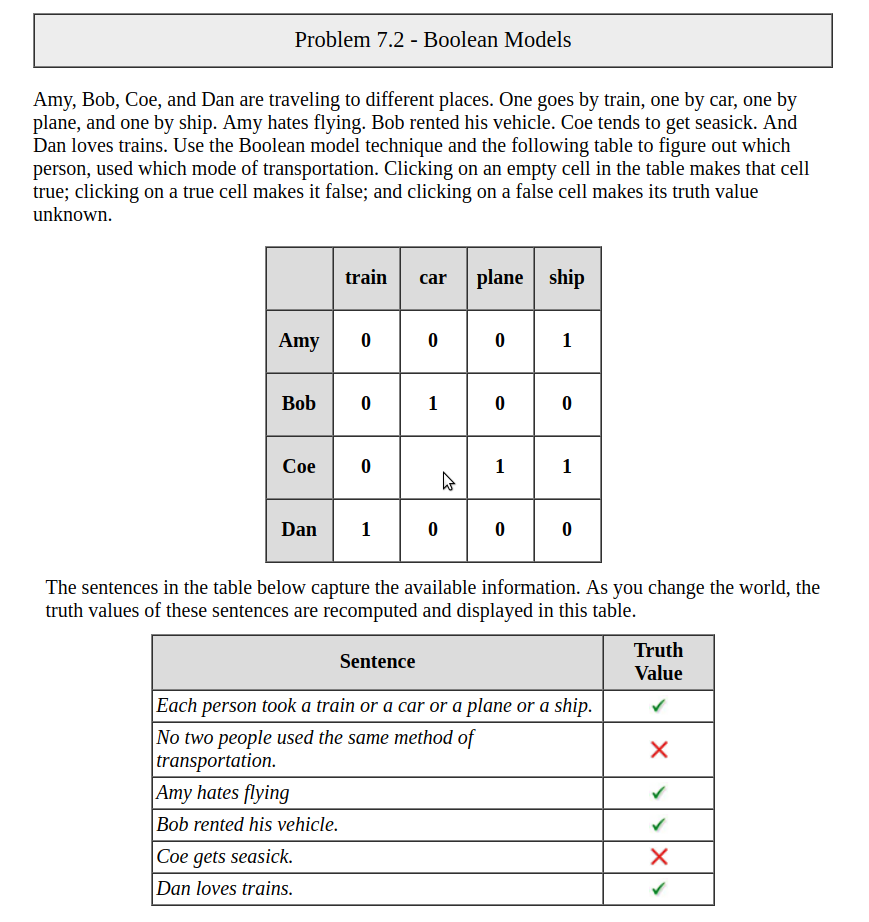
\includegraphics[scale=0.4]{relacna-tabulka-hodnota-formuly}
	\caption{Hľadanie kombinácie kedy sú všetky vety pravdivé.}
	\label{fig:fixne-formuly}
\end{figure}

\begin{figure}[h]
	\centering
	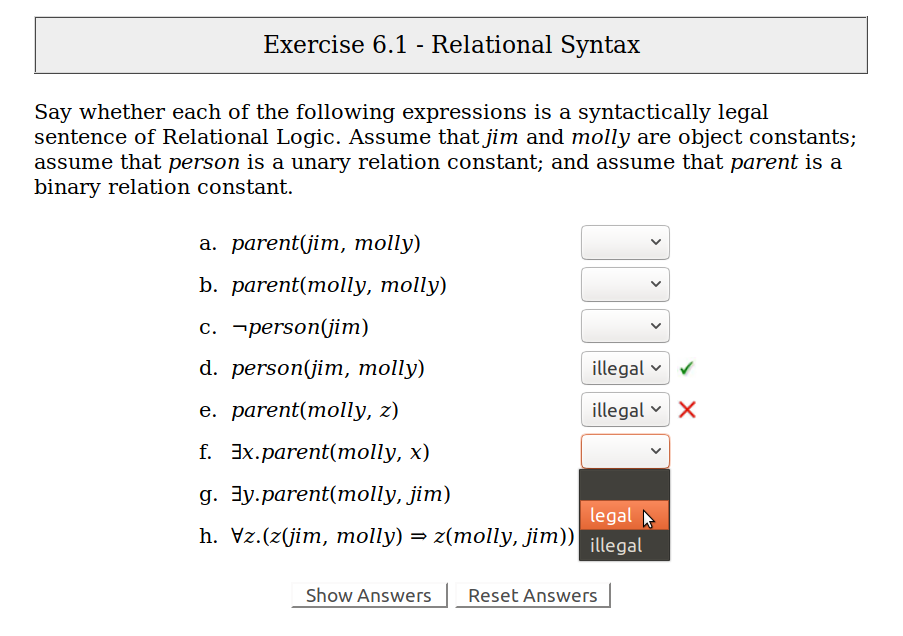
\includegraphics[scale=0.4]{syntax}
	\caption{Cvičenie zamerané na precvičovanie syntaxe.}
	\label{fig:syntax}
\end{figure}

\begin{figure}[h]
	\centering
	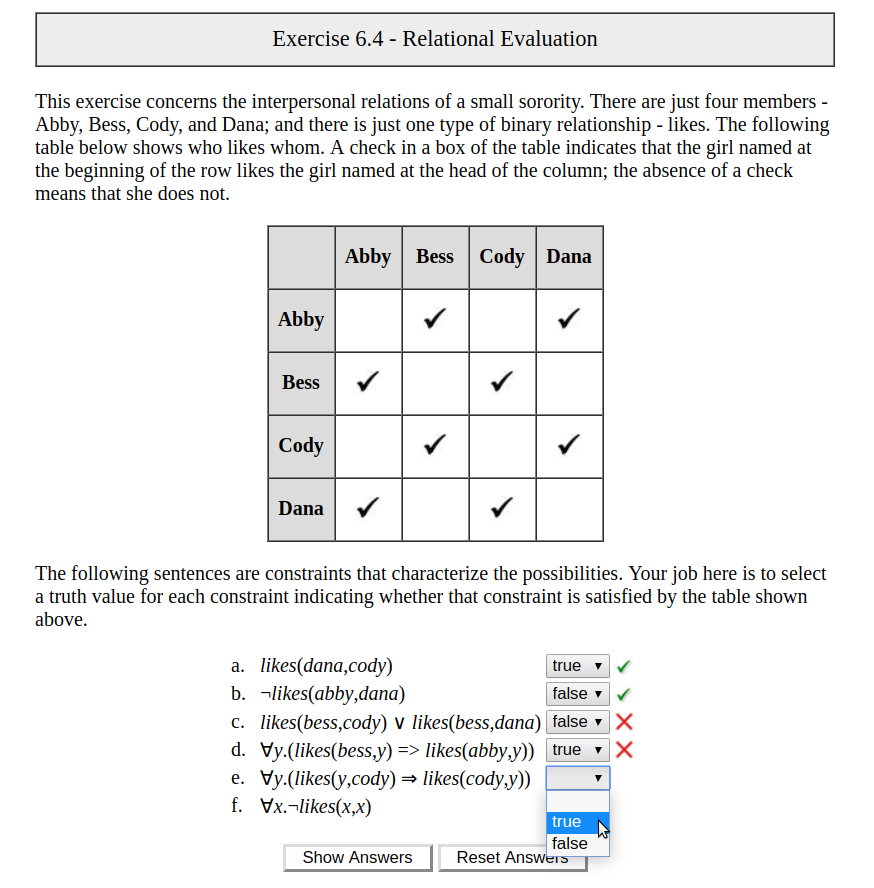
\includegraphics[scale=0.4]{hodnota-predikatu-2}
	\caption{Hľadanie pravdivostnej hodnoty formuly pri danej fixnej tabuľke pravdivostných hodnôt predikátu \texttt{likes}.}
	\label{fig:hodnota-predikatu-2}
\end{figure}




\subsection{Logický pracovný stôl}
Bakalárska práca s názvom \emph{Logický pracovný stôl} \cite{lps} sa zaoberá výrokovou logikou. Výsledkom tejto práce je aplikácia, ktorá ponúka užívateľovi interaktívne pracovať s formulami výrokovej logiky, vie zistiť, či je formula splniteľná, nesplniteľná, alebo či je to tautológia. Podobne ako pri mojej práci, obsahuje vstup, kde sa dá zapísať ľubovoľná formula. Tento vstup sa následne sparsuje a napríklad zistiť, či je to tautológia alebo nie.

\subsection{Výukový program demonštrujúci matematický princíp}
Druhá bakalárska práca ktorá sa zaoberá metematickou logikou je \emph{Výukový program demonštrujúci matematický princíp} \cite{vpdmp}. Práca sa zaoberá tvorbou webovej aplikácie, kde si užívateľ precvičuje postupy matematických dôkazov. Konkrétne sa zaoberá dokazovaním rovnosti viet Boolovej algebry. Užívateľ si dôkaz konkrétnej pred-pripravenej vety vo forme rovnice môže vyskladať pomocou axióm. 
